\chapter{\MSTlong{} Methodology}\label{chap:methodology}
There are two main components we investigated for the purpose of \mst{}: 
clustering for \bslongs{}
and
the \kraplong{} (\krap{}).
The clustering method we use is based off of the density-based clustering algorithm \dbscan, as introduced in \autoref{sec:dbscan} and described in \cite{johnson2015density}.
The \krap{} derives its classification ability from \kNNlong{}, outlined in \autoref{sec:knn}, adding four methods to resolve the multiple \knnlong{} lists that are a product of multiple neighbor-\compfuncs{} and an \a{} threshold to filter the \knnlong{} lists.
This Chapter describes the use of these two methods as classification methodologies for \cplop{}.

\section{Clustering for Bacterial Strains}\label{sec:clusteringbs}
For the purposes of this work, we define an \ecoli{} strain as a \textit{group of \ecoli{} isolates that share exactly the same \Ssixt{} and \Sfive{} DNA sequences.}

From the computer science point of view, a bacterial strain is essentially a cluster of \ecoli{} \isol{} representations stored in \cplop{}.
Our \mst{} method, thus, works as follows:
\begin{enumerate}
    \item \textbf{Strain Identification.} Identify bacterial strains in \cplop{} by clustering
    all \cplop{} \isols{}.
    \item \textbf{MST.} Given an isolate of unknown origin, find the cluster it belongs to.
    Return the \spec{} of the plurality of isolates in the cluster.
\end{enumerate}

For our clustering algorithm, we use a density-based clustering algorithm
developed by Johnson \cite{johnson2015density}. This algorithm extends DBSCAN
for the case of two similarity metrics between data points (our isolates are compared
based on two ITS regions) and implements an efficient spatial data structure to manage
the storage and retrieval of the data points.

In this paper we look at the results of clustering \cplop{} data using this algorithm from the perspective of \textit{cluster purity}. We call a cluster (strain) \textit{100\% pure}
if all isolates that belong to it come from the same \spec{}. 

Of interest to us is the following information:
\begin{enumerate}
    \item The number of 100\% pure clusters and the percentage of bacterial isolates from \cplop{} clustered into pure clusters.
    \item The structure of impure clusters: specifically, whether a dominant \spec{} can
    be clearly identified in each cluster.
    \item Coverage: the total number of \cplop{} isolates found to belong to a strain.
    \item MST Accuracy: the percentage of isolates for which the strain-based MST procedure produces the correct response.
\end{enumerate}

In the next section we provide a brief discussion of the density-based clustering algorithm
of Johnson \cite{johnson2015density} and its use to build \cplop{} \isol{} clusters.


\section{\krap{}}\label{sec:krap}

In order to accommodate these separate similarity metrics, we need a resolution procedure.
Rather than creating a new similarity metric out of a pair of similarity scores, we choose to update the \kNN{} method with four different ways of selecting the resultant category label based on how the pyroprints compare to each other. 
These four methods are described below.

In what follows, we generalize our problem. Given \UNKNOWN{} and \KNOWN{}, two library objects (\isols{}), and a collection of \compfuncs{}, \COMP{}$=(\COMP{}_1,\ldots \COMP{}_m)$, with $m > 1$, comparing \UNKNOWN{} to \KNOWN{} gives us a collection of values:  
$\COMP{}(\UNKNOWN{},\KNOWN{}) = (\COMP{}_1(\UNKNOWN{},\KNOWN{}),\ldots,\COMP{}_m(\UNKNOWN{},\KNOWN{}))$.
All four resolution procedures described in this section work with such a generalized representation of \isols{} and \compfuncs{} between them.

Given an unknown \isol{} \UNKNOWN{}, a library of classified\footnote{A ``classified \isol{}'' is an \isol{} for which the \spec{} has been identified in the database.} \isols{} \LIB{}, and a set of \compfuncs{} \COMP{}, we compare \UNKNOWN{} to each object in \LIB{} using each \compfunc{} in \COMP{}. To resolve these \compfuncs{}, we propose four algorithms:

\subsection{Comparing \Isols{}}
Of primary interest to the biologists using \cplop{} is comparing \isols{} to each other. In \cplop{}, each \isol{} is represented by a pair of mutually incomparable \pyros{}: one for each of the two \itsshort{} regions.
As a result, given \isols{} $I_1, I_2$, we can represent each as a pair of pyroprint vectors 
\[I_1 = (\vec{q}_1, \vec{q}_2) \text{ and } I_2 = (\vec{r}_1, \vec{r}_2),
\]
where $\vec{q}_1 \text{ and } \vec{r}_1$ are respectively $I_1 \text{ and } I_2$'s \Ssixt{} \pyro{} and $\vec{q}_2 \text{ and } \vec{r}_2$ are respectively $I_1 \text{ and } I_2$'s \Sfive{} \pyro{} \cite{Black2014121}. Since \pyro{}s from different regions are incomparable, comparing \isol{}s must be done as follows:
\[
\COMP{}(I_1, I_2) = (\pcfunclabel(\vec{q}_1, \vec{r}_1), \pcfunclabel(\vec{q}_2, \vec{r}_2)),
\]
where $\pcfunclabel(\cdot,\cdot)$ is between \pyros{} of the same \itsshort{} region and is the \pearson{}. Thus, when comparing \isol{}s, we effectively have two different similarity metrics, one for each \itsshort{} region:
\[
\COMP{}(I_1, I_2) = (\COMPsixt{}(I_1, I_2), \COMPfive{}(I_1, I_2)).
\]

\begin{algorithm}[H]
\caption{Isolate Comparison Metric}\label{alg:compare}
\textit{Input}:
    \begin{itemize}
    \item $u\in\ISOL{}$: an \isol{}
    \item $v\in\ISOL{}$: an \isol{}
    \end{itemize}
\textit{Output}:
    \begin{itemize}
    \item \R{} value, indicating similarity
    \end{itemize}
\textit{Requires}:
    \begin{itemize}
    \item Each \isol{} has a \pyro{} in the $i^{th}$ ITS region
    \end{itemize}

\begin{algorithmic}[1]
\Procedure{$C_i(u,v)$}{}
\State $\vec{p_u} \leftarrow$ \Call{GetPyroprint$_i$}{$u$}
\State $\vec{p_v} \leftarrow$ \Call{GetPyroprint$_i$}{$v$}
\State \Return \Call{PearsonCorrelation}{$\vec{p_u},\vec{p_v}$}
\EndProcedure
\end{algorithmic}
\end{algorithm}

\subsection{\a{} Filtering}
Our first modification to \kNN{} is an additional condition at step \ref{knn:filter}:
\begin{enumerate}
\setcounter{enumi}{3}
\item Consider only the top $k$ entries in $N$ above threshold $\alpha$
\end{enumerate}

The $\alpha$ threshold allows biologists to filter out neighbors that are among the $k$ closest, but too dissimilar to compare. 
When comparing multiple \pyro{}s of the same region of a single \isol{}, the Pearson Correlation between them is strictly above 0.99.
As a result, for many other studies --- not necessarily MST-focused --- a Pearson Correlation of 0.99 or above is used to define a strain of \ecoli{}. 
Filtering by some value near this may give more accurate results and provides an intuitive way to relate these lists to other studies.
\begin{algorithm}[H]
\caption{\kNN{} with $\alpha$ Threshold}\label{alg:filter}
\textit{Input}:
    \begin{itemize}
    \item $list$: sorted list
    \end{itemize}
\textit{Output}:
    \begin{itemize}
    \item $nearest$: the top $k$ elements above the threshold $\alpha$
    \end{itemize}
\textit{Requires}:
    \begin{itemize}
    \item $k$ and $\alpha$ are predetermined
    \item each element in $list$ has a similarity field $sim$
    \end{itemize}

\begin{algorithmic}[1]
\Procedure{Filter$_{k, \alpha}$}{$list$}
\State $nearest\gets\emptyset$
\State $i\gets0$
\While{$i < k$ \textbf{and} $list[i].sim < \alpha$}
\State \add{$list[i]$}{$nearest$}
\State $i\gets i + 1$
\EndWhile
\State\Return{$nearest$}
\EndProcedure
\end{algorithmic}
\end{algorithm}

\subsection{\rmean{}}
For $U$ and a $P\in\LIB{}$, we take the mean of the result of all of the \compfuncs{} and build a single \knnlong{} list from it.
The mean can be any metric mapping $\R^n\times\R^n\rightarrow\R$ and in the investigated implementation, we use the euclidean distance, also known as the $L^2$ norm.
A single \knnlong{} list results from this algorithm that we filter by $k$ and $\alpha$ and use to classify the unknown.
\autoref{alg:mean} describes this process in pseudocode.
\begin{algorithm}[H]
\caption{\rmean}\label{alg:mean}

\textit{Input}:
\begin{itemize}
\item $u\in\UNKN{}$: an unknown \isol{}
\item $\LIB{}\subseteq\ISOL{}$: a library of known \isol{}s
\end{itemize}
\textit{Output}:
\begin{itemize}
\item \SPEC{} value, classifying the unknown \isol{} $u$
\end{itemize}
\textit{Requires}:
\begin{itemize}
\item $k$, $\alpha$, and the set of comparison metrics \COMP{} are predetermined
\end{itemize}

\begin{algorithmic}[1]
\Procedure{ClassifyMean$(u,\LIB)$}{}
\State$N \gets\emptyset$    \COMMENT[.6]{Make nearest neighbors list.}
\For{$p\in\LIB$}            \COMMENT[.6]{For each library element:}
\State$\AVG{}\gets\{\emptyset\}$    \COMMENT[.55]{Make empty set for results.}
    \For{$C_i\in \COMP{}$}          \COMMENT[.55]{For each comparison metric:}
    \State $sim\gets$ \Call{$C_i$}{$u,p$}   \COMMENT[.3]{Compare.}
    \State \add{$sim$}{\AVG{}}              \COMMENT[.3]{Track result.}
    \EndFor
    \State $mean\gets $\Call{Mean}{\AVG{}}  \COMMENT[.47]{Mean the results.}
    \State \add{$(mean,p)$}{$N$}          \COMMENT[.47]{Add mean to neighbors.}
\EndFor
\State \sort{$N$}{$sim$}      \COMMENT[.5]{Sort by most similar.}
\State $N\gets$\Call{Filter$_{k,\alpha}$}{$N$} \COMMENT[.5]{Keep the nearest.}
\State$s\gets$ \Call{FindMostPluralSpecies}{$M$}
\State\Return $s$
\EndProcedure
\end{algorithmic}
\end{algorithm}

\subsection{\rwinner{}}
For each \compfunc{}, we make a \knnlong{} list and filter by $k$ and $\alpha$ accordingly.
Once we finish building each \compfunc{}'s \knn{} list, we find the most plural classification from each list and track the number of times that classification shows up in that list.
Then, we classify $u$ based off the classification that has the highest number in its corresponding list.
\autoref{alg:winner} describes this process in pseudocode.
\begin{algorithm}[H]
\caption{\rwinner}\label{alg:winner}

\textit{Input}:
\begin{itemize}
\item $u\in\UNKN{}$: an unknown \isol{}
\item $\LIB{}\subseteq\ISOL{}$: a library of known \isol{}s
\end{itemize}
\textit{Output}:
\begin{itemize}
\item \SPEC{} value, classifying the unknown \isol{} $u$
\end{itemize}
\textit{Requires}:
\begin{itemize}
\item $k$, $\alpha$, and the set of comparison metrics \COMP{} are predetermined
\end{itemize}

\begin{algorithmic}[1]
\Procedure{ClassifyWinner$(u,\LIB)$}{}
\State $N\gets\emptyset$\COMMENT[.6]{New list to track neighbor lists.}
\For{$C_i\in \COMP{}$}                \COMMENT[.6]{For each comparison metric:}
\State$N_i \gets\emptyset$      \COMMENT[.55]{Make nearest neighbors list.}
    \For{$p\in\LIB$}            \COMMENT[.55]{For each library element:}
    \State $sim\gets$ \Call{$C_i$}{$u,p$}   \COMMENT{Compare.}
    \State \add{$(sim,p)$}{$N_i$}           \COMMENT{Add to neighbors.}
    \EndFor
    \State \sort{$N_i$}{$sim$}                          \COMMENT[.45]{Sort by most similar.}
    \State $N_i\gets$\Call{Filter$_{k,\alpha}$}{$N_i$} \COMMENT[.45]{Keep the nearest.}
    \State \add{$N_i$}{$N$}
\EndFor
\State $S\gets\{\emptyset\}$ \COMMENT[.6]{To track each list's most plural.}
\For{$N_i\in N$}
\State$s\gets$ \Call{FindMostPluralSpecies}{$N_i$}
\State\add{$s$}{$S$}
\EndFor
\State\Return \Call{Max}{$S$}\COMMENT[.6]{The most plural overall.}
\EndProcedure
\end{algorithmic}
\end{algorithm}

\subsection{\runion{}}
For each \compfunc{}, we make a \knnlong{} list and filter by $k$ and $\alpha$ accordingly.
After building each \knnlong{} list, we combine the lists into a set, keeping track of the original list position for tie-breaking.
From this set, which we dub the union, we count the classifications present in the union and classify $u$ as the most plural in the union of the lists, compared to the other lists.
\autoref{alg:union} describes this process in pseudocode.
\begin{algorithm}[H]
\caption{\runion}\label{alg:union}

\textit{Input}:
\begin{itemize}
\item $u\in\UNKN{}$: an unknown \isol{}
\item $\LIB{}\subseteq\ISOL{}$: a library of known \isol{}s
\end{itemize}
\textit{Output}:
\begin{itemize}
\item \SPEC{} value, classifying the unknown \isol{} $u$
\end{itemize}
\textit{Requires}:
\begin{itemize}
\item $k$, $\alpha$, and the set of comparison metrics \COMP{} are predetermined
\end{itemize}

\begin{algorithmic}[1]
\Procedure{ClassifySetwise$(u,\LIB)$}{}
\State $\MERG{}\gets\{\emptyset\}$    \COMMENT[.6]{Create new common set.}
\For{$C_i\in \COMP{}$}                \COMMENT[.6]{For each comparison metric:}
\State$N_i \gets\emptyset$      \COMMENT[.55]{Make nearest neighbors list.}
    \For{$p\in\LIB$}            \COMMENT[.55]{For each library element:}
    \State $sim\gets$ \Call{$C_i$}{$u,p$}   \COMMENT{Compare.}
    \State \add{$(sim,p)$}{$N_i$}           \COMMENT{Add to neighbors.}
    \EndFor
    \State \sort{$N_i$}{$sim$}    \COMMENT[.55]{Sort by most similar.}
    \State $N_i\gets$\Call{Filter$_{k,\alpha}$}{$N_i$} \COMMENT[.45]{Keep the nearest.}
    \For{$n\in N_i$}            \COMMENT[.55]{For each nearest neighbor:}
    \State \add{$n$}{\MERG{}}\COMMENT{Add to common set.}
    \EndFor
\EndFor
\State$s\gets$ \Call{FindMostPluralSpecies}{$M$}
\State\Return $s$
\EndProcedure
\end{algorithmic}
\end{algorithm}

\subsection{\rintersect{}}
For each \compfunc{}, we make a \knnlong{} list and filter by $k$ and $\alpha$ accordingly, but ensure that we do not lose track of the entire sorted list of results.
After building each \knnlong{} list, we inspect each list for common \isol{}s.
We add \isol{}s that appear in every list into a set that we call the intersection.
If the size of the intersection is $k$, then we are done.
Otherwise, we increase the length of our individual lists by $\delta$ and search for common \isol{}.
This process repeats until the size of the intersection is $k$, or all of the \isol{}s in the individual lists are below threshold $\alpha$.
\autoref{alg:intersection} describes this process in pseudocode.
\begin{algorithm}[H]
\caption{\rintersect{}}\label{alg:intersection}

\textit{Input}:
\begin{itemize}
\item $u\in\UNKN{}$: an unknown \isol{}
\item $\LIB{}\subseteq\ISOL{}$: a library of known \isol{}s
\end{itemize}
\textit{Output}:
\begin{itemize}
\item \SPEC{} value, classifying the unknown \isol{} $u$
\end{itemize}
\textit{Requires}:
\begin{itemize}
\item $k$, $\alpha$, $\delta$, and the set of comparison metrics \COMP{} are predetermined
\end{itemize}

\begin{algorithmic}[1]
\Procedure{ClassifyIntersection$(u,\LIB)$}{}
\State $N\gets\emptyset$\COMMENT[.6]{New list to track neighbor lists.}
\For{$C_i\in \COMP{}$}                \COMMENT[.6]{For each comparison metric:}
\State$N_i \gets\emptyset$      \COMMENT[.55]{Make nearest neighbors list.}
    \For{$p\in\LIB$}            \COMMENT[.55]{For each library element:}
    \State $sim\gets$ \Call{$C_i$}{$u,p$}   \COMMENT{Compare.}
    \State \add{$(sim,p)$}{$N_i$}           \COMMENT{Add to neighbors.}
    \EndFor
    \State \sort{$N_i$}{$sim$}    \COMMENT[.45]{Sort by most similar.}
    
    \State \add{$N_i$}{$N$}
\EndFor
\State $done\gets$ false
\While{$\neg done$}
\For{$N_i\in N$}
\State $N_i'\gets\emptyset$
\State $N_i'\gets$\Call{Filter$_{k,\alpha}$}{$N_i$}
\EndFor

\If{$|N_1'\cap\dots\cap N_n'| < k$}
\State $k\gets k + \delta$
\Else
\State $N_\cap\gets N_1'\cap\dots\cap N_n'$ 
\State $done\gets$ true
\EndIf
\EndWhile
\State\Return \Call{FindMostPluralSpecies}{$N_\cap$}
\EndProcedure
\end{algorithmic}
\end{algorithm}

\subsection{\cplop{} Makeup}
\autoref{fig:species} shows the distribution of \cplop{} \isols{} considered in this study among its 53 different \spec{}.
\begin{figure}[t]
    \centering
    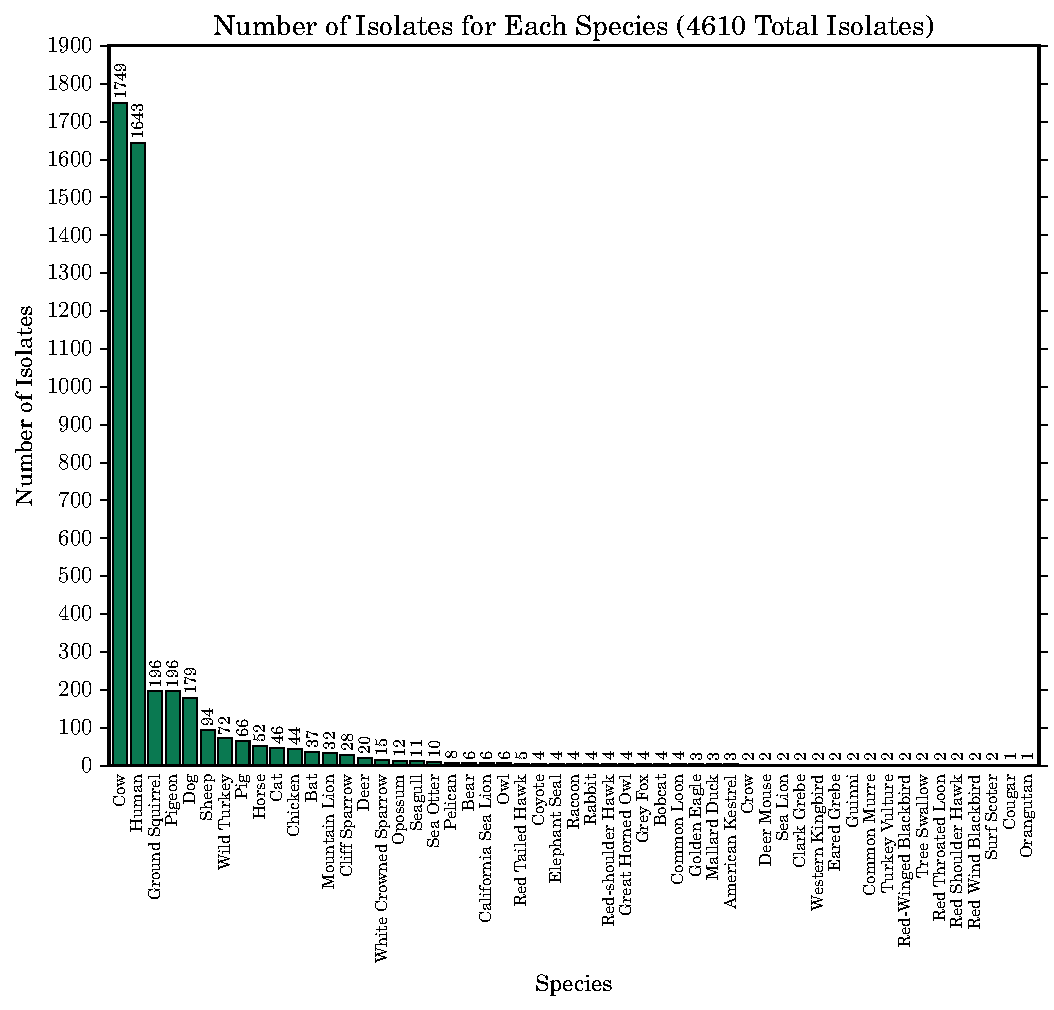
\includegraphics[width=\linewidth]{figures/bs/species_hist.pdf}
    \caption{
    A histogram of the number of \isols{} of each species in our study, taken from \cplop{}.
    There are 4,610 total \isols{} from 53 different \specs{}.}
    \label{fig:species}
\end{figure}

There are a total of 4,610 \isols{} in our dataset\footnote{A simplified version of \cplop{} containing \isol{} IDs, \spec{}, and \zscore{}s can be found at \texttt{https://github.com/jmcgover/cplop-acm-bcb-2016}.}. As seen from Figure \ref{fig:species},
the organic growth of \cplop{} yielded disproportionately many \ecoli{} isolates originating
from humans and cows (however, as shall be seen below, these isolates belong to a large number of strains). Each \isol{} is represented in \cplop{} with two \pyros{} ---  one each for \its{1} and \its{2} 
region.
